\documentclass[runningheads,a4paper]{llncs}
%
\usepackage{natbib} % bibliography stuff
%
\usepackage{graphicx} % allows for working with images
\DeclareGraphicsExtensions{.pdf,.png,.jpeg,.jpg,.gif} % configures latex to look for the following image extensions
%
\usepackage{setspace} % allows for configuring the linespacing in the document
%\singlespacing
\onehalfspacing
%\doublespacing
%
\usepackage{listings}
%
\usepackage{amsmath}
%
\usepackage{appendix}
%
\usepackage{multirow}
%
\usepackage{booktabs,array,dcolumn}
%
\usepackage{float}
%
\usepackage{eurosym}
%
\usepackage{caption}
\captionsetup[table]{skip=10pt}
\captionsetup{compatibility=false}
\usepackage{subcaption}
%
\usepackage[toc]{glossaries}
\makeglossaries
%
\usepackage{amssymb}
\setcounter{tocdepth}{4}
%
\usepackage{url}
\urldef{\mailsa}\path|info@southeastmakerspace.org|
\newcommand{\keywords}[1]{\par\addvspace\baselineskip
\noindent\keywordname\enspace\ignorespaces#1}

%Optional Package to add PDF bookmarks and hypertext links
\usepackage[pdftex,hypertexnames=false,linktocpage=true]{hyperref}
\hypersetup{colorlinks=true,linkcolor=black,anchorcolor=black,citecolor=black,filecolor=black,urlcolor=black,bookmarksnumbered=true,pdfview=FitB}

\begin{document}
\mainmatter  % start of an individual contribution

% first the title is needed
\title{An Introduction to Arduino \\a low cost digital prototyping platform}

% a short form should be given in case it is too long for the running head
\titlerunning{Introduction to Arduino}
%

% the name(s) of the author(s) follow(s) next
%
% Chinese authors should write their first names(s) in front of
% their surnames. This ensures that the names appear correctly in
% the running heads and the author index.
%
\author{Clive Barry%
%\thanks{Please note that the LNCS Editorial assumes that all authors have used
%the western naming convention, with given names preceding surnames. This determines
%the structure of the names in the running heads and the author index.}%
\and Mogue Carpenter \and Aileen Drohan \and David Kirwan \and Martin Walshe}
%
\authorrunning{Introduction to Arduino}
% (feature abused for this document to repeat the title also on left hand pages)

% the affiliations are given next; don't give your e-mail address
% unless you accept that it will be published
\institute{South East Makerspace,\\Old Printworks, Thomas Hill,\\Waterford City, X91 TW63\\
\mailsa\\
\url{https://www.southeastmakerspace.org}}
%

%
% a more complex sample for affiliations and the mapping to the
% corresponding authors can be found in the file "llncs.dem"
% (search for the string "\mainmatter" where a contribution starts).
% "llncs.dem" accompanies the document class "llncs.cls".
%
%\toctitle{Thesis Proposal}
\tocauthor{SEMS}
\maketitle

%
\begin{abstract}
\begin{figure}
	\centering
	
\includegraphics[width=8cm]{images/sems}
\end{figure}
This workshop offers an introduction to the Arduino prototyping platform, useful for artists, hobbiests and the wider maker community. Each participant receives a pack containing an Arduino Uno and components to perform each of 5 simple experiments. No prior coding experience is needed as all code will be provided. The only requirement is the Arduino IDE, and a packed lunch!
\keywords{arduino, digital electronics, prototyping, introduction}
\end{abstract}
%

%%%%%%%%%%%%%%%%%%%%%%%%%%%%%%%%%%%%%%%%%%%%%%%%%%%%%%%%%%%%%%%%%%%%%%%%%%%%%%%%%%%%%%%%%%%%%%%%%%%
%% Acknowledgements
%\newpage
%\chapter*{Acknowledgements}
I'd like to thank my legs, for always supporting me; my arms, who are always by my side and lastly my fingers, I can always count on them.

%

%
\tableofcontents
%

%
%\newpage
%\listoffigures
%\addcontentsline{toc}{chapter}{List of Figures}
%

%
%\newpage
%\listoftables
%\addcontentsline{toc}{chapter}{List of Tables}

%%%%%%%%%%%%%%%%%%%%%%%%%%%%%%%%%%%%%%%%%%%%%%%%%%%%%%%%%%%%%%%%%%%%%%%%%%%%%%%%%%%%%
%

%
\newpage
\chapter*{Introduction}
\addcontentsline{toc}{chapter}{Introduction}

\section*{What is an Arduino?}
\addcontentsline{toc}{section}{What is an Arduino?}

"Over the years \gls{Arduino} has been the brain of thousands of projects, from everyday objects to complex scientific instruments. A worldwide community of makers - students, hobbyists, artists, programmers, and professionals - has gathered around this open-source platform, their contributions have added up to an incredible amount of accessible knowledge that can be of great help to novices and experts alike."~\citep{arduino-15-a} 

%
\begin{figure}[ht]
	\centering
	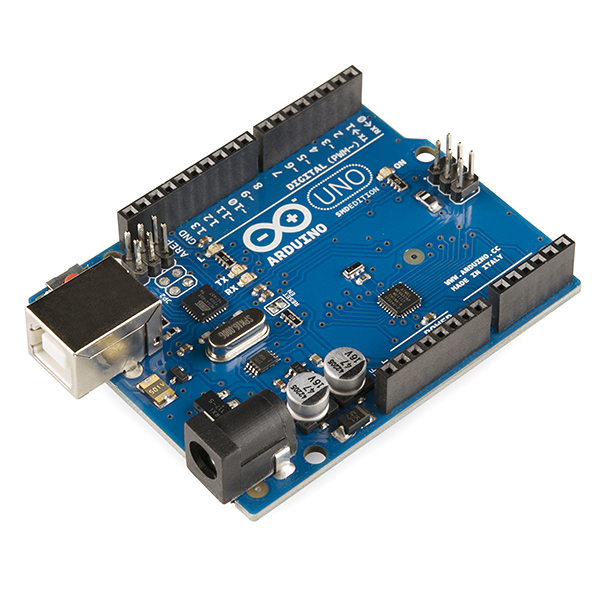
\includegraphics[width=8cm]{images/01}
	\caption{Arduino Uno R3 \citep{wikipedia-13}}
	\label{fig:arduino_uno_r3}
\end{figure}
%


\begin{description}
	\item[Open Source] \hfill \\
	Open Source can be described as resources and software that can be used, redistributed, rewritten and in some circumstances sold free of charge. The schematics and component list for hardware can also be open source as is the case with the \gls{Arduino} platform~\citep{culkin-11}.
	
	\item[Electronics] \hfill \\
	Technology which makes use of the controlled motion of electrons through different media~\citep{culkin-11}.
	
	\item[Prototype] \hfill \\
	An original form that can serve as a basis or standard for other things~\citep{culkin-11}.
	
	\item[Platform] \hfill \\
	Hardware architecture with software framework on which other software can run~\citep{culkin-11}.
\end{description}

\section*{Where might an Arduino be used?}
\addcontentsline{toc}{section}{Where might an Arduino be used?}
A few contrived examples of where one might use an Arduino in order to automate some process:

\subsection*{Automatic Dog's Water Bowl}
An dog owner wants to ensure her pet is never left without water. She attaches a system for measuring the water level in the dog's bowl. Her \gls{Arduino} is programmed to measure this value every 5 minutes. If this level falls below a certain value, a valve is opened and a water pump is activated to fill up the water bowl. It then sends an SMS to the owner to let her know that the dog is in safe hands.

\begin{itemize}
	\item Read inputs from a water level sensor
	\item Control a valve which lets water flow
	\item Control speed of a water pump 
	\item Send SMS to owner about giving the dog water
\end{itemize}

\subsection*{Bird Table Camera}
A rising social media ornithologist wishes to share pictures from all the visitors to the bird table in his garden. He mounts an infra-red movement sensor on the bird table attached to an \gls{Arduino} which is configured to record an image and send it to Twitter. His neighbours marvel at how many crows he's feeding.

\begin{itemize}
	\item Read inputs from a movement sensor
	\item Control a camera shutter
	\item Transmit image back to PC
	\item Send tweet with picture of the bird table visitor
\end{itemize}

\subsection*{Fingerprint Door Lock}
A student is sick of forgetting his keys and being locked out of his house. He uses a fingerprint scanner and an Arduino to make a biometric fingerprint door lock. He needs only scan his thumb print now and the door will unlock.

\begin{itemize}
	\item Read inputs from a fingerprint sensor
	\item Compares the finger print against an authorised fingerprint
	\item Records the time and date a finger was pressed on the scanner
	\item Makes audio error tone if the fingerprint was invalid
	\item If valid fingerprint it unlocks the door
\end{itemize}

%
\begin{figure}[ht]
	\centering
	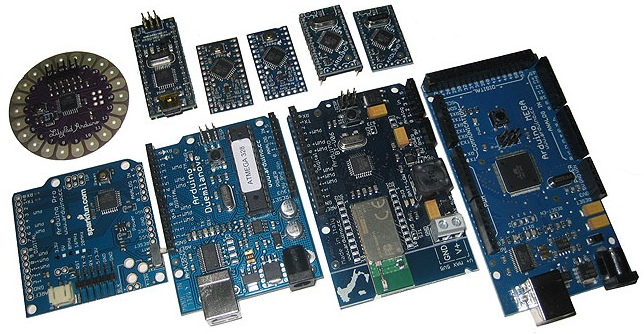
\includegraphics[width=12cm]{images/10}
	\caption{Arduino Family}
	\label{fig:arduino_family}
\end{figure}
%

There are multiple different flavours of \gls{Arduino}, each with different capability levels and or specialised features. It is through this variety which makes it is possible to use the Arduino in a wide range of situations from home automation to wearable technology.

\newpage
\section*{Workshop Aims}
\addcontentsline{toc}{section}{Workshop Aims}
In this workshop the aim is to give you a crash course in digital electronics, and provide you with the basic skill-set to start using the Arduino or similar micro-controllers in your future projects.

\begin{description}
	\item[Workshop Requirements] \hfill \\
	Each person will require the following:
	\begin{itemize}
		\item PC, either Linux, Mac or Windows can be used
		\item Arduino IDE pre-installed (Internet at the makerspace is flaky!)
		\item A sambo to keep you going
	\end{itemize}
	
	\item[Learning Outcomes] \hfill \\
	Each person will leave with:
	\begin{itemize}
		\item Arduino starter kit
		\item Crash course in digital electronics
		\item Confidence to use Arduino in future projects
	\end{itemize}
\end{description}

\subsection*{Arduino Starter Kit Contents}
The Arduino starter kit contains the following components, which we will be making use of during the workshop.

\begin{itemize}
	\item 1 $\times$ Arduino Compatible R3 Uno
	\item 1 $\times$ Breadboard
	\item 16 $\times$ jumper wires various colours
	\item 20 $\times$ 5mm LED's assorted colours
	\item 10 $\times$ 10k$\Omega$ resistors
	\item 10 $\times$ 330$\Omega$ resistors
	\item 1 $\times$ RGB LED
	\item 1 $\times$ photo resistor
	\item 2 $\times$ push buttons
	\item 1 $\times$ DFRobot MP3 Module
	\item 1 $\times$ 1GB SD Card
	\item 1 $\times$ 5$\Omega$ speaker
\end{itemize}


\newpage
\section*{Basic Circuit Theory}
\addcontentsline{toc}{section}{Basic Circuit Theory}

In an electrical circuit there is a fundamental relationship between voltage, current and resistance and it is explained by Ohm’s Law~\citep{et-15}.

\subsection*{Voltage}
Voltage, (SI Unit: $V$ - Volts) is the potential energy of an electrical supply stored in the form of an electrical charge. Voltage can be thought of as the force that pushes electrons through a conductor and the greater the voltage the greater is its ability to push the electrons through a given circuit~\citep{et-15}.

%
\begin{figure}[ht]
	\centering
	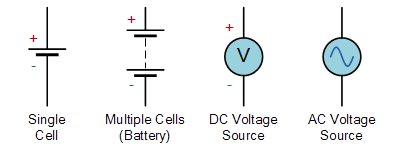
\includegraphics[width=7cm]{images/02}
	\caption{Voltage Symbols \citep{et-15}}
	\label{fig:voltage_symbols}
\end{figure}
%

\subsection*{Current}
Current, (SI Unit: $A$ - Ampere) is the movement or flow of electrical charge and is measured in Amperes. It is the continuous and uniform flow (called a drift) of electrons (the negative particles of an atom) around a circuit that are being pushed by the voltage source~\citep{et-15}.

%
\begin{figure}[ht]
	\centering
	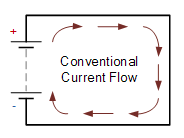
\includegraphics[width=4cm]{images/03}
	\caption{Current Symbols \citep{et-15}}
	\label{fig:current_symbols}
\end{figure}
%

\newpage
\subsection*{Resistance}
Resistance, (SI Unit: $\Omega$ - Ohms) of a circuit is its ability to resist or prevent the flow of current (electron flow) through itself making it necessary to apply a greater voltage to the electrical circuit to cause the current to flow again. Note that Resistance cannot be negative in value only positive~\citep{et-15}.

%
\begin{figure}[ht]
	\centering
	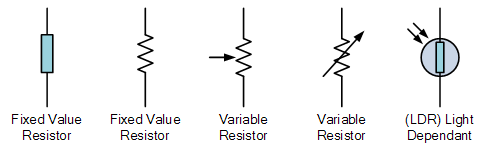
\includegraphics[width=8cm]{images/04}
	\caption{Resistance Symbols \citep{et-15}}
	\label{fig:resistance_symbols}
\end{figure}
%

\subsection*{Ohm's Law}
The following equation Ohm's Law explains the relationship between Voltage, Current and Resistance for an electrical circuit. For more information see:~\citep{et-14}.

%
\begin{figure}[ht]
	\centering
	\begin{equation}
	V = I \times R
	\end{equation}
	\begin{equation}
	I = \frac{V}{R}
	\end{equation}
	\begin{equation}
	R = \frac{V}{I} 
	\end{equation}
	\caption{Ohm's Law}
	\label{fig:ohms_law_equation}
\end{figure}
%


\subsection*{Analogue vs Digital Signals}

The world we live in is an analogue one. There are an infinite number of possible combinations of colours smells and sounds. The digital world however is not infinite. It is discrete and finite where we are limited by several factors, such as memory and computational capabilities. In order to represent a real world thing digitally, it is by necessity that some information is lost.

\begin{description}
	\item[Analogue Signal Examples] \hfill \\
	The following are some examples of analogue signals:
	\begin{itemize}
		\item Temperature
		\item Sound
		\item EM Radiation
	\end{itemize}
	%
	\begin{figure}[ht]
		\centering
		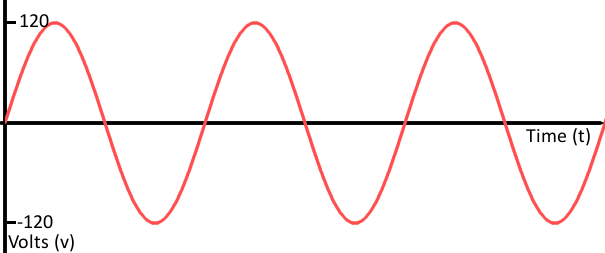
\includegraphics[width=8cm]{images/05}
		\caption{Analogue Signal \citep{lindblom-15}}
		\label{fig:analogue_signal}
	\end{figure}
	%
	
	\item[Digital Signal Examples] \hfill \\
	The following are some examples of digital signals:
	\begin{itemize}
		\item Morse Code
		\item WIFI
		\item Binary
	\end{itemize}
	%
	\begin{figure}[ht]
		\centering
		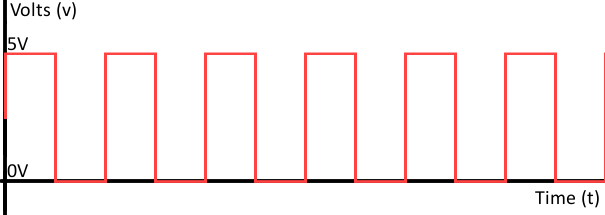
\includegraphics[width=8cm]{images/06}
		\caption{Digital Signal \citep{lindblom-15}}
		\label{fig:digital_signal}
	\end{figure}
	%
\end{description}





\newpage
\section*{Electronic Components}
\addcontentsline{toc}{section}{Electronic Components}
The following section contains more information on some of the various components included in the \textit{Introduction to Arduino} workshop. 

%
\begin{figure}[ht]
	\centering
	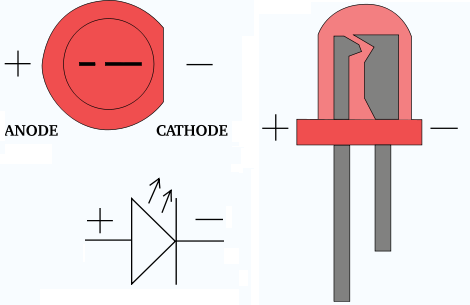
\includegraphics[width=08cm]{images/16}
	\caption{LED Component \citep{sapkota-10}}
	\label{fig:led_component}
\end{figure}
%

%
\begin{figure}[ht]
	\centering
	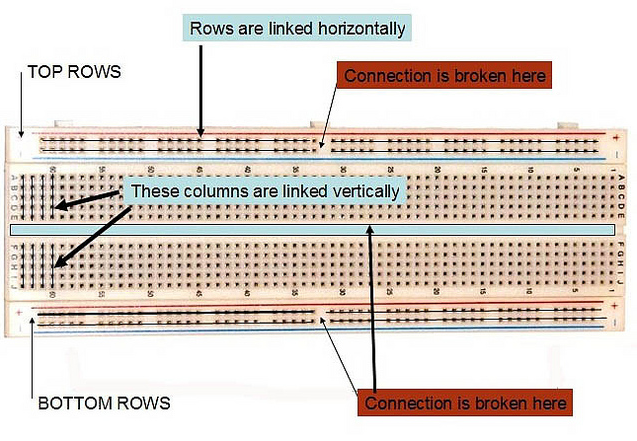
\includegraphics[width=08cm]{images/17}
	\caption{Breadboard \citep{sapkota-10}}
	\label{fig:breadboard_component}
\end{figure}
%

%
\begin{figure}[ht]
	\centering
	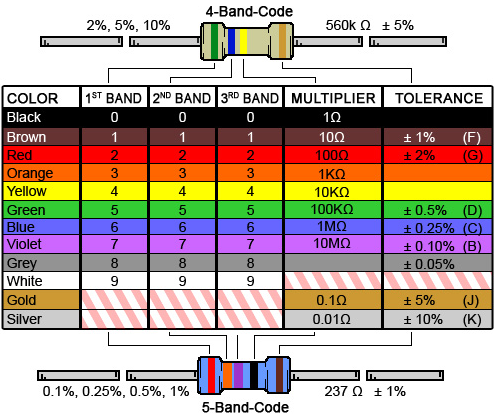
\includegraphics[width=08cm]{images/18}
	\caption{Resistor Chart \citep{digikey-16}}
	\label{fig:resistor_component}
\end{figure}
%




\newpage
\section*{Basic Arduino Coding Concepts}
\addcontentsline{toc}{section}{Basic Arduino Coding Concepts}


\begin{description}
	\item[Variables] \hfill \\
	A variable is a way of naming and storing a value for later use by the program, such as data from a sensor or an intermediate value used in a calculation~\citep{arduino-15-b}.
	%
	\begin{table}
		\centering
		\begin{tabular}{p{4cm} l}
			\toprule
			Type & Example\\ \midrule
			char & 'a' \\
			string & 'Hello there' \\
			byte & 0 to 255 \\
			int & -32,768 to 32,767 \\
			unsigned int & 0 to 65,535 \\
			long & -2,147,483,648 to 2,147,483,647 \\
			unsigned long & 0 to 4,294,967,295 \\
			float & -3.4028235E38 to 3.4028235E38 \\
			\bottomrule
		\end{tabular}
		\caption{Variable Types in Wiring}
		\label{tab:wiring_variable_types}
	\end{table}
	%
	Table:~\ref{tab:wiring_variable_types} shows some of the basic variable types available to us for use in the Arduino. There are other more advanced data types such as Arrays and Pointers, which we may use, but won't explain them in this introduction. More information can be found regarding these data types online. See the Arduino online reference library at: https://www.arduino.cc/en/Reference/HomePage.
	
	\item[setup() function] \hfill \\
	The setup() function is called when a sketch starts. Use it to initialize variables, pin modes, start using libraries, etc. The setup function will only run once, after each power-up or reset of the Arduino board~\citep{arduino-15-c}.
	%
	\begin{lstlisting}

void setup(){ // setup initializes serial
  Serial.begin(9600);
}
void loop(){ // write to serial, then wait 2 seconds
  Serial.write("Hello World");
  delay(2000);
}
	\end{lstlisting}
	%

\newpage	
	\item[loop() function] \hfill \\
	After creating a setup() function, which initializes and sets the initial values, the loop() function does precisely what its name suggests, and loops consecutively, allowing your program to change and respond. Use it to actively control the Arduino board~\citep{arduino-15-d}.
	%
	\begin{lstlisting}
// Create int variable to represent
// a physical pin on the Arduino
int buttonPin = 3;

// setup initializes serial and the button pin
void setup()
{
  Serial.begin(9600);
  pinMode(buttonPin, INPUT);
}

// loop checks the button pin each time,
// and will send serial if it is pressed
void loop()
{
  if (digitalRead(buttonPin) == HIGH)
    Serial.write('H');
  else
    Serial.write('L');
  
  delay(1000);
}
	\end{lstlisting}
	%	
\end{description}
\chapter*{Experiment 1 - Blink}
\addcontentsline{toc}{chapter}{Experiment 1 - Blink}
This example is what one might call the \textit{hello world} example for \gls{Arduino} sketches. We wire up the experiment as shown in the diagram fig:~\ref{fig:exp1_blink}. And upload the \gls{Sketch} code in the next section on page:~\pageref{sketch:exp1}.

%
\begin{figure}[ht]
	\centering
	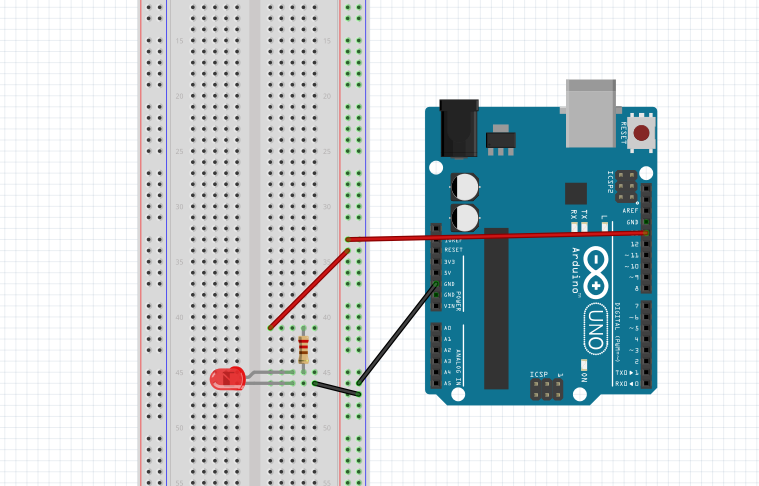
\includegraphics[width=12cm]{images/07}
	\caption{LED Blink \citep{fritzing-15}}
	\label{fig:exp1_blink}
\end{figure}
%

When the Arduino boots, the led should flash on for a second, then off for a second and repeat.

\newpage
\section*{Sketch Code}
\label{sketch:exp1}
\begin{lstlisting}
/*
Blink
Turns on an LED on for one second, then off for one second, repeatedly.

This example code is in the public domain.
*/

// the setup function runs once when you press reset or power the board
void setup() {
  // initialize digital pin 13 as an output.
  pinMode(13, OUTPUT);
}

// the loop function runs over and over again forever
void loop() {
  // turn the LED on 
  // (HIGH is the voltage level)
  digitalWrite(13, HIGH);
	
  //wait for 1000 milliseconds
  delay(1000);
	
  // turn the LED off by making 
  // the voltage LOW
  digitalWrite(13, LOW);    
	            
  // wait for 1000 milliseconds              
  delay(1000);
}
\end{lstlisting}
\chapter*{Experiment 2 - Button}
\addcontentsline{toc}{chapter}{Experiment 2 - Button}
We wire up the experiment as shown in the diagram fig:~\ref{fig:exp2_button}. And upload the sketch code in the next section on page:~\pageref{sketch:exp2}.

%
\begin{figure}[ht]
	\centering
	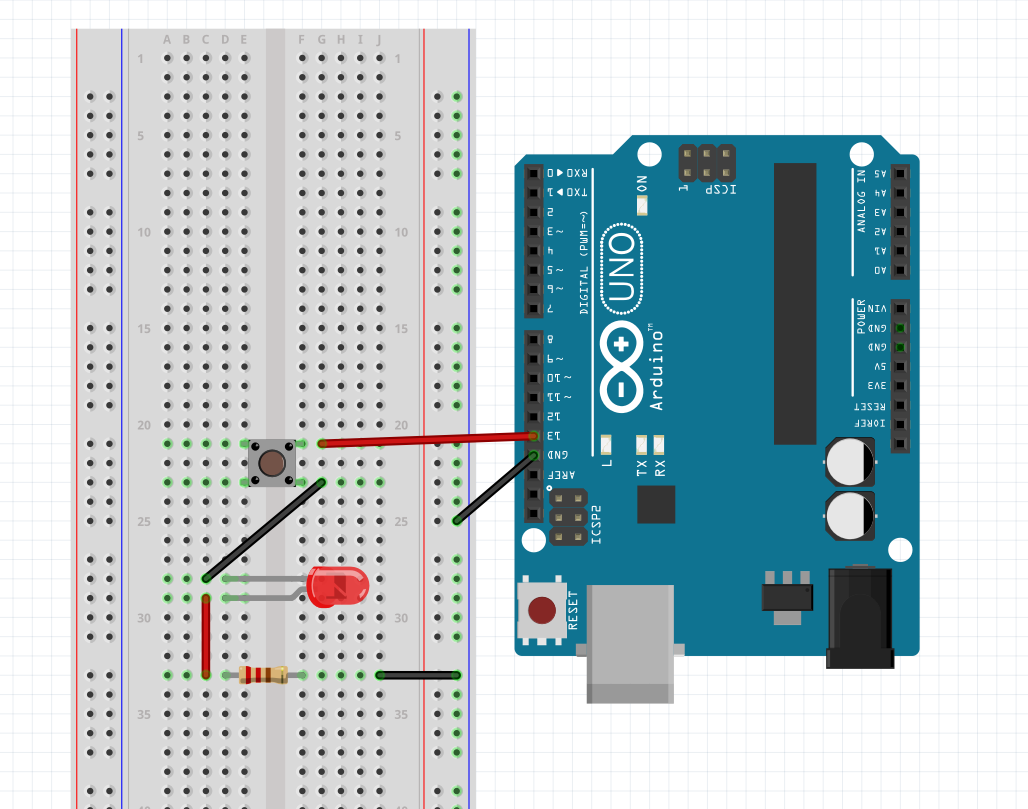
\includegraphics[width=12cm]{images/08}
	\caption{Button activated LED \citep{fritzing-15}}
	\label{fig:exp2_button}
\end{figure}
%

The LED will light up when the button is pressed.

\newpage
\section*{Sketch Code}
\label{sketch:exp2}
\begin{lstlisting}
/*
Button activated LED

This example code is in the public domain.
*/

 
// Pin 13 has an LED connected on most Arduino boards.
// give it a name:
int led = 13;

// the setup routine runs once when you press reset:
void setup() {                
  // initialize the digital pin as an output.
  pinMode(led, OUTPUT);     
}

// the loop routine runs over and over again forever:
void loop() {
  digitalWrite(led, HIGH);   // turn the LED on (HIGH is the voltage level)
}

\end{lstlisting}
\chapter*{Experiment 3 - Generating Music}
\addcontentsline{toc}{chapter}{Experiment 3 - Generating Music}
We wire up the experiment as shown in the diagram fig:~\ref{fig:exp3_music}. And upload the sketch code in the next section on page:~\pageref{sketch:exp3}.

%
\begin{figure}[ht]
	\centering
	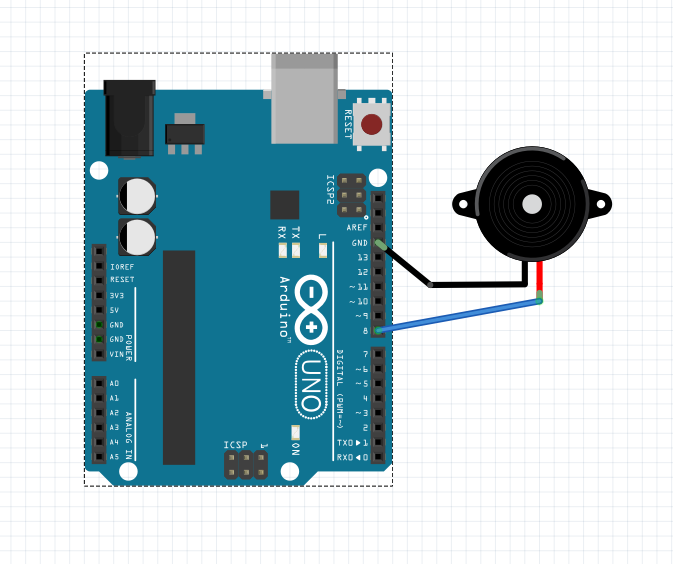
\includegraphics[width=12cm]{images/09}
	\caption{Play musical notes through a speaker \citep{fritzing-15}}
	\label{fig:exp3_music}
\end{figure}
%

As soon as the \gls{Arduino} boots it should play a series of musical notes and then stop. For more information see the online reference page for the functions used in this experiment here: https://www.arduino.cc/en/Reference/Tone

\newpage
\section*{Sketch Code}
\label{sketch:exp3}
\begin{lstlisting}
/*
Melody - Plays a melody
This example code is in the public domain.
*/
#include "pitches.h"

int melody[] = { // notes in the melody:
  NOTE_C4, NOTE_G3, NOTE_G3, NOTE_A3, NOTE_G3, 0, NOTE_B3, NOTE_C4
};

// note durations: 4 = quarter note, 8 = eighth note, etc.:
int noteDurations[] = {
  4, 8, 8, 4, 4, 4, 4, 4
};

void setup() {
  // iterate over the notes of the melody:
  for (int thisNote = 0; thisNote < 8; thisNote++) {
    // to calculate the note duration, take one second
    // divided by the note type.
    //e.g. quarter note = 1000 / 4, eighth note = 1000/8, etc.
    int noteDuration = 1000 / noteDurations[thisNote];
    tone(8, melody[thisNote], noteDuration);
    // to distinguish the notes, set a minimum time between them.
    // the note's duration + 30% seems to work well:
    int pauseBetweenNotes = noteDuration * 1.30;
    delay(pauseBetweenNotes);
    noTone(8);
  }
}

void loop() {
  // no need to repeat the melody.
}

// ********************* pitches.h ************************

/*************************************************
* Public Constants
*************************************************/

#define NOTE_B0  31
#define NOTE_C1  33
#define NOTE_CS1 35
#define NOTE_D1  37
#define NOTE_DS1 39
#define NOTE_E1  41
#define NOTE_F1  44
#define NOTE_FS1 46
#define NOTE_G1  49
#define NOTE_GS1 52
#define NOTE_A1  55
#define NOTE_AS1 58
#define NOTE_B1  62
#define NOTE_C2  65
#define NOTE_CS2 69
#define NOTE_D2  73
#define NOTE_DS2 78
#define NOTE_E2  82
#define NOTE_F2  87
#define NOTE_FS2 93
#define NOTE_G2  98
#define NOTE_GS2 104
#define NOTE_A2  110
#define NOTE_AS2 117
#define NOTE_B2  123
#define NOTE_C3  131
#define NOTE_CS3 139
#define NOTE_D3  147
#define NOTE_DS3 156
#define NOTE_E3  165
#define NOTE_F3  175
#define NOTE_FS3 185
#define NOTE_G3  196
#define NOTE_GS3 208
#define NOTE_A3  220
#define NOTE_AS3 233
#define NOTE_B3  247
#define NOTE_C4  262
#define NOTE_CS4 277
#define NOTE_D4  294
#define NOTE_DS4 311
#define NOTE_E4  330
#define NOTE_F4  349
#define NOTE_FS4 370
#define NOTE_G4  392
#define NOTE_GS4 415
#define NOTE_A4  440
#define NOTE_AS4 466
#define NOTE_B4  494
#define NOTE_C5  523
#define NOTE_CS5 554
#define NOTE_D5  587
#define NOTE_DS5 622
#define NOTE_E5  659
#define NOTE_F5  698
#define NOTE_FS5 740
#define NOTE_G5  784
#define NOTE_GS5 831
#define NOTE_A5  880
#define NOTE_AS5 932
#define NOTE_B5  988
#define NOTE_C6  1047
#define NOTE_CS6 1109
#define NOTE_D6  1175
#define NOTE_DS6 1245
#define NOTE_E6  1319
#define NOTE_F6  1397
#define NOTE_FS6 1480
#define NOTE_G6  1568
#define NOTE_GS6 1661
#define NOTE_A6  1760
#define NOTE_AS6 1865
#define NOTE_B6  1976
#define NOTE_C7  2093
#define NOTE_CS7 2217
#define NOTE_D7  2349
#define NOTE_DS7 2489
#define NOTE_E7  2637
#define NOTE_F7  2794
#define NOTE_FS7 2960
#define NOTE_G7  3136
#define NOTE_GS7 3322
#define NOTE_A7  3520
#define NOTE_AS7 3729
#define NOTE_B7  3951
#define NOTE_C8  4186
#define NOTE_CS8 4435
#define NOTE_D8  4699
#define NOTE_DS8 4978
\end{lstlisting}
\chapter*{Experiment 4 - Thermistor}
\addcontentsline{toc}{chapter}{Experiment 4 - Thermistor}
We wire up the experiment as shown in the diagram fig:~\ref{fig:exp4_thermistor}. And upload the sketch code in the next section on page:~\pageref{sketch:exp4}.

%
\begin{figure}[ht]
	\centering
	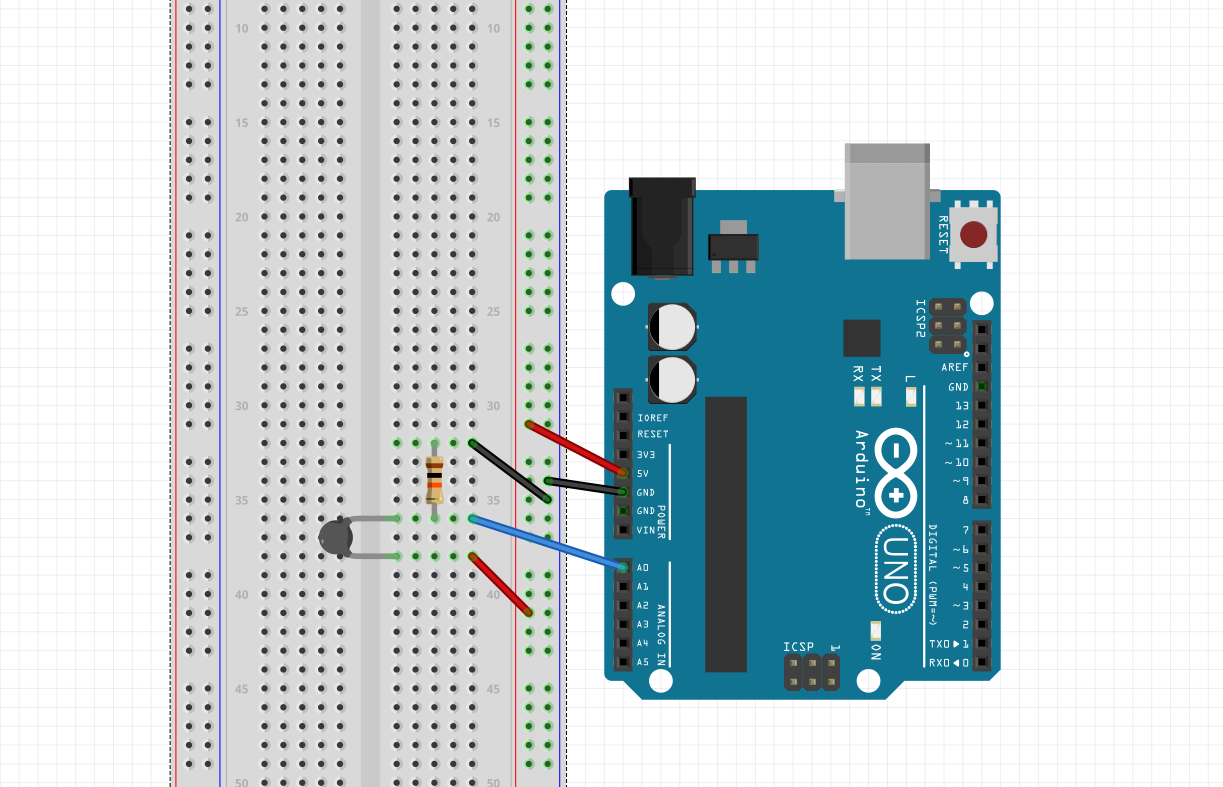
\includegraphics[width=12cm]{images/19}
	\caption{Read a Thermistor Value}
	\label{fig:exp4_thermistor}
\end{figure}
%

The thermistor is an electrical resistor whose resistance is greatly reduced by heating. Its often used for measurement and control applications. The following graph fig:~\ref{fig:exp4_thermistor_plot} on page:~\pageref{fig:exp4_thermistor_plot}. demonstrates the fall of resistance as the temperature rises.

To view the values being read from the thermistor, simply open the Arduino serial monitor.

%
\begin{figure}[ht]
	\centering
	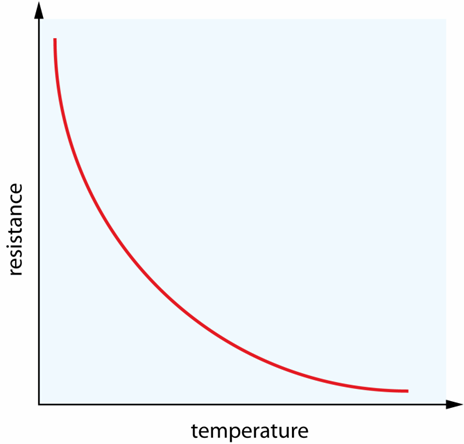
\includegraphics[width=12cm]{images/20}
	\caption{Thermistor Plot: Resistance vs Temperature}
	\label{fig:exp4_thermistor_plot}
\end{figure}
%

\newpage
\section*{Sketch Code}
\label{sketch:exp4}
\begin{lstlisting}
/*
Sample code to work with a Thermistor

Author: David Kirwan
Licence: Apache 2.0
*/

int sensorPin = A0;
int sensorValue = 0;

void setup() {
  // declare the ledPin as an OUTPUT:
  Serial.begin(9600);
  pinMode(sensorPin, INPUT);
}

void loop() {
  // read the value from the sensor:
  sensorValue = analogRead(sensorPin);
  Serial.println(sensorValue);
  delay(sensorValue);
}
\end{lstlisting}
\chapter*{Experiment 5 - clap4Led}
\addcontentsline{toc}{chapter}{Experiment 5 - clap4Led}
We wire up the experiment as shown in the diagram fig:~\ref{fig:exp5_microphone}. And upload the sketch code in the next section on page:~\pageref{sketch:exp5}.

%
\begin{figure}[ht]
	\centering
	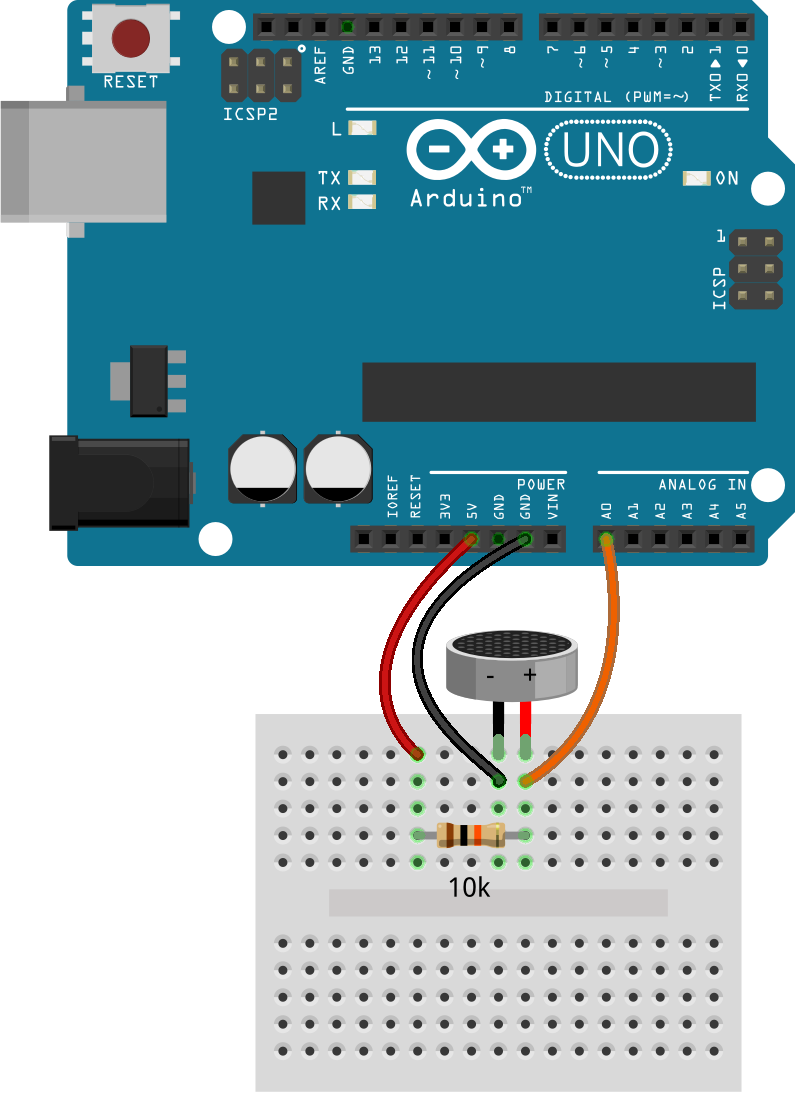
\includegraphics[width=8cm]{images/21}
	\caption{Microphone Activated Circuit}
	\label{fig:exp5_microphone}
\end{figure}
%

The microphone module is polarised, which means it has a positive and negative terminal which must be correctly placed in the circuit in order to function as expected. Please examine the diagram fig:~\ref{fig:exp5_microphone_polarity} on page:~\pageref{fig:exp5_microphone_polarity} to correctly identify which leg is positive and which is negative.

When this circuit is complete, the LED onboard the Arduino will flash when the microphone detects sound.

%
\begin{figure}[ht]
	\centering
	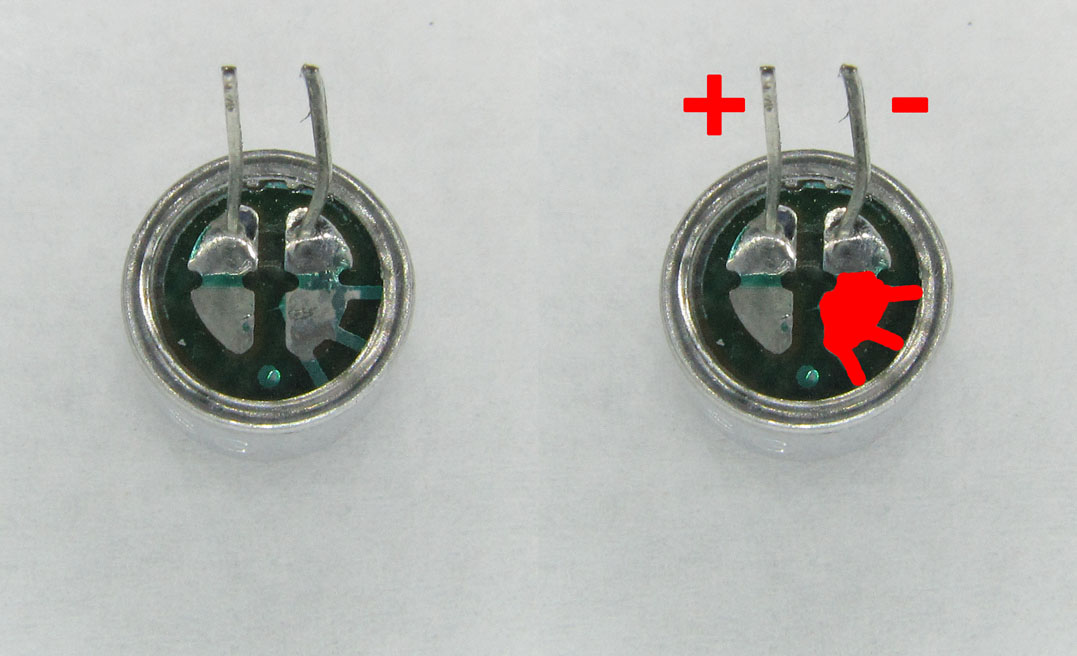
\includegraphics[width=12cm]{images/22}
	\caption{Microphone Module Polarity}
	\label{fig:exp5_microphone_polarity}
\end{figure}
%


\newpage
\section*{Sketch Code}
\label{sketch:exp5}
\begin{lstlisting}
/*
<<<<<<< HEAD
Sample code to work with a Thermistor

Author: Anton Krug
Licence: Apache 2.0
*/

//global variables
int readValue;
int maximumValue;
int minimumValue; 


// will reset maximum and minimum values only when we call it
void resetMaximumAndMinimum() 
{
  maximumValue = 0;             // set maximum to lowest value possible
  minimumValue = 32767;         // set minimum to highest value possible
}


// this runs only once on the startup
void setup() 
{
  // initialize built-in LED light at digital pin 13 as an output
  pinMode(13, OUTPUT);           
  resetMaximumAndMinimum();
}


// the loop runs over and over again forever
void loop() 
{
  // read current value from the microphone
  readValue = analogRead(A0);     

  // if read value is smaller than minimum then set it as the new minimum
  if (readValue < minimumValue)   
  {
    minimumValue = readValue;     
  }

  // if read value is bigger than maximum then set it as the new maximum
  if (readValue > maximumValue)   
  {
    maximumValue = readValue;     
  }

  // Change the 10 constant to adjust the sensitivity.
  //   To 20 if you want the light triggered on louder claps   
  //   Ti 5  if you want the light triggered on quieter noises 
  //   Feel free to experiment with the values.
  if ( (maximumValue - minimumValue) > 10 ) 
  {
    digitalWrite(13, HIGH);       // turn the LED on (HIGH is the voltage level)
    delay(2 * 1000);              // wait for 2 seconds (2 * 1000ms)
    digitalWrite(13, LOW );       // turn the LED off by making the voltage LOW

    // if we wouldn't clear the max & min then after first trigger it would get 
    // triggered every single time no matter what read values were
    resetMaximumAndMinimum();     
  }
}

=======
Phenakistoscope
Turns on an LED on then off 20 times a second in order to activate the Phenakistoscope
*/

// the setup function runs once when you press reset or power the board
void setup() {
  // initialize digital pin 13 as an output.
  pinMode(13, OUTPUT);
}

// the loop function runs over and over again forever
void loop() {
  // turn the LED on 
  // (HIGH is the voltage level)
  digitalWrite(13, HIGH);
	
  //wait for 10 milliseconds
  delay(10);
	
  // turn the LED off by making 
  // the voltage LOW
  digitalWrite(13, LOW);    
	            
  // wait for 30 milliseconds              
  delay(30);
}
>>>>>>> 0581ff186ec5408b185455777b58f0f20d96f775
\end{lstlisting}
\newpage
\chapter*{Thanks for taking part!}
\addcontentsline{toc}{chapter}{Thanks for taking part!}

Do you want to know more? Of course you do! \citet{fried-12} has developed a number of tutorials suitable for the beginner wishing to learn more about the \gls{Arduino} system. These tutorials can be accessed at the following URI: http://www.ladyada.net/learn/arduino/

Would you like to work on or with technology like this in the future? Would you like to change profession? Then you might also be interested in investigating the newly formed \textit{Internet of Things} degree course being run at the Waterford Insstitute of Technology: https://www.wit.ie/courses/school/science/department\_of\_computing\_maths\_physics/bsc-hons-in-the-internet-of-things

I hope you enjoyed this workshop and your time spent here. The South East Makerspace have developed a number of workshops in this space and are in the process of designing more. Be sure to sign up to the mailing list, and follow us on social media!  We would be delighted to welcome new faces, however full membership is restricted to over 18's for insurance reasons! For information on SEMS see:

\begin{description}
	\item[Facebook] http://www.facebook.com/SouthEastMakerSpace
	\item[FAQ] https://wiki.southeastmakerspace.org/faq
	\item[Google+] http://plus.google.com/u/0/108025738894009906004/
	\item[How to join] https://wiki.southeastmakerspace.org/how\_to\_join\_sems
	\item[Mailing List] http://lists.southeastmakerspace.org/mailman/listinfo/sems-general
	\item[Secure Contact] https://www.southeastmakerspace.org/contact
	\item[Twitter] http://twitter.com/SEMakerSpace
\end{description} 





%

%
%%%%%%%%%%%%%%%%%%%%%%%%%%%%%%%%%%%%%%%%%%%%%%%%%%%%%%%%%%%%%%%%%%%%%%%%%%%%%%%%%%%%%
%
%
\newglossaryentry{Arduino}
{
  name={Arduino},
  description={an open-source electronics platform based on easy-to-use hardware and software. It's intended for anyone making interactive projects. https://www.arduino.cc},
  sort=Arduino
}
%

%
\newglossaryentry{LED}
{
	name={LED},
	description={a light emitting diode is a p-n junction diode which emits light when activated. https://en.wikipedia.org/wiki/Light-emitting\_diode},
	sort=LED
}
%

%
\newglossaryentry{Sketch}
{
	name={Sketch},
	description={a sketch is the name that Arduino uses for a program. Once compiled the resulting firmware can be installed on the Arduino device. https://www.arduino.cc/en/Tutorial/Sketch},
	sort=Sketch
}
%
\renewcommand*{\glsclearpage}{}
\printglossaries
%

%
%\appendix
%\chapter*{Appendix}
\addcontentsline{toc}{chapter}{Appendices}

%

%
\bibliographystyle{plainnat}
\bibliography{bibliography/bibtex}
\addcontentsline{toc}{chapter}{Bibliography}
%

\end{document}


